\section{SGX Memory Organization}
\label{sec:memory}

The central concept of SGX is the \textit{enclave}, a protected environment
that contains the code and data pertaining to a security-sensitive computation.
This section provides an overview of the data structures used by an enclave.


\subsection{Enclaves in DRAM}
\label{sec:prm}

% PRM: SGX/SGX2 S 3.5
% Interactions with DMA: SGX/SGX2 S 6.10
% Interactions with Memory Configuration: SGX/SGX2 S 6.11

The enclaves' code and data is stored in \textit{Processor Reserved Memory}
(PRM), which cannot be directly accessed by other software, including system
software and SMM code. The CPU's integrated memory controllers
(\S~\ref{sec:cpu_die}) also reject DMA transfers targeting the PRM, thus
protecting it from access by other peripherals.

\begin{figure}[hbt]
  \centering
  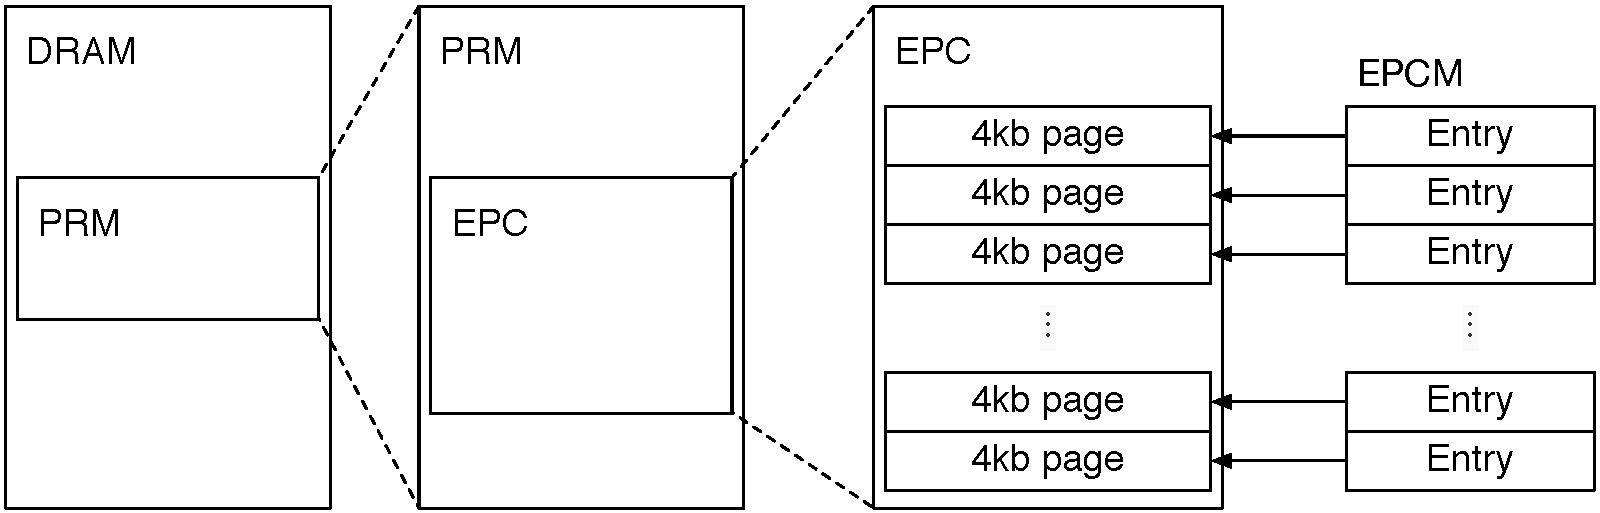
\includegraphics[width=87mm]{figures/sgx_epc.pdf}
  \caption{
    Enclave data is stored into the EPC, which is a subset of the PRM. The
    PRM is a contiguous range of DRAM that cannot be accessed by system
    software or peripherals.
  }
  \label{fig:sgx_epc}
\end{figure}

The PRM range is configured using a base and a mask register with the same
semantics as a variable memory type range (\S~\ref{sec:cacheability_config}),
which implies that the PRM's size must be an integer power of two, and its
start address must be aligned to the same power of two. These restrictions make
it cheap to check if an address belongs to the PRM in hardware, as described in
\S~\ref{sec:cacheability_config}.


\subsubsection{The Enclave Page Cache (EPC)}
\label{sec:epc}

% EPC and EPCM: SGX/SGX2 S 1.5, S 1.5.1, S 3.5, S 3.5.1
%               SGX S 2.6.13, SGX2 S 2.6.19

The contents of enclaves and the associated data structures are stored in the
\textit{Enclave Page Cache} (EPC), which is a subset of the PRM.

The SGX design supports having multiple enclaves on a system at the same time,
which is a  necessity in multi-process environments. This is achieved by having
the EPC split into 4~KB pages that can be associated to different enclaves. The
system software uses SGX instructions to allocate unused pages to enclaves, and
to free previously allocated EPC pages.

The SGX instructions that allocate an EPC page to an enclave also copy data
from a page outside PRM to the EPC page. Non-enclave software is not permitted
to access the PRM, so the page allocation instructions are the only avenue for
system software to load the initial code and data into an enclave.

SGX also offers a method for system software to evict EPC pages into non-PRM
memory, which allows the EPC to be over-committed, just like evicting DRAM
pages to disk (swapping) allows the main memory to be over-committed.


\subsubsection{Memory Mapping Attacks}
\label{sec:mapping_attacks}

% Access Control Requirements: SGX/SGX2 S 2.3

One of SGX's design goals is to make it easy to migrate the sensitive pieces of
an application into an enclave. To this end, enclave code uses the same address
translation process (\S~\ref{sec:paging}) as the application hosting the
enclave. It follows that enclave code can access non-EPC memory using the same
virtual addresses as the host application, which makes it easy to migrate
application code that uses pointers into SGX enclaves.

% Interactions with VMX: SGX/SGX2 S 6.5, 6.5.{1,2,3,4,5}

Under SGX, the operating system and hypervisor are still in full control of the
page tables and EPTs. This minimizes the amount of changes required to add SGX
support to existing system software. However, it also gives system software the
ability to attack an enclave by setting up its virtual address space in a way
that was not intended by the enclave's author.

Figure~\ref{fig:sgx_mapping_attack} shows a hypothetical memory mapping attack
that is prevented by SGX's security measures. Understanding this type of attack
greatly increases one's ability to reason about SGX's security.

\begin{figure}[hbt]
  \centering
  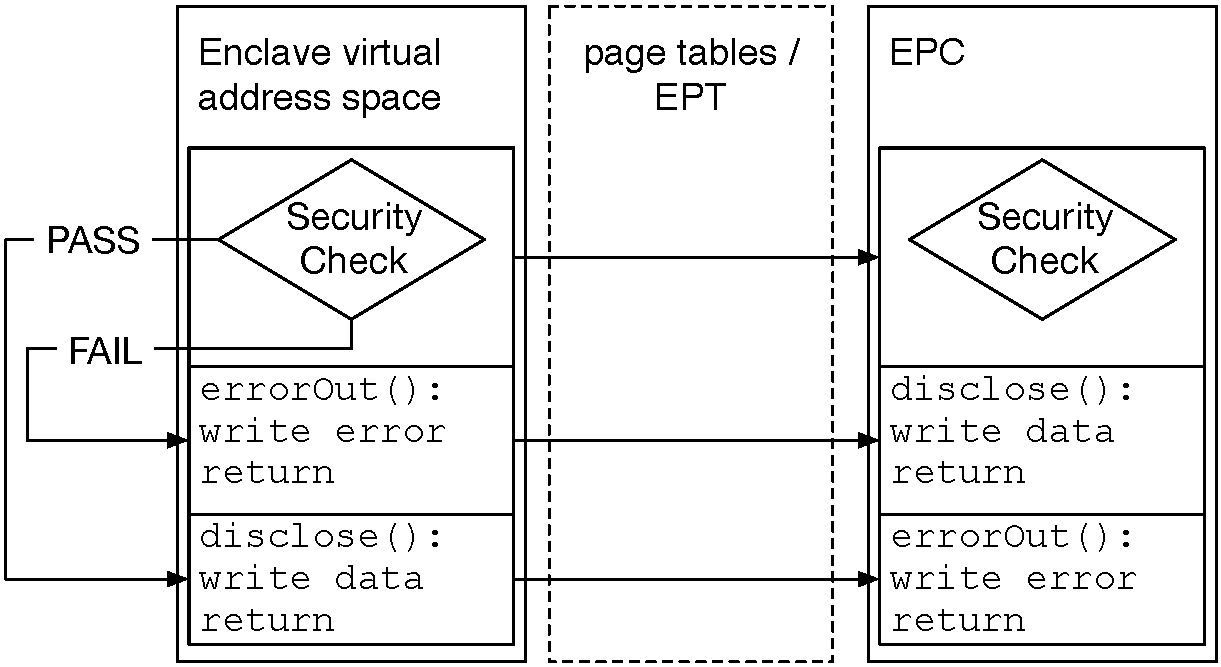
\includegraphics[width=85mm]{figures/sgx_mapping_attack.pdf}
  \caption{
    An example of a memory mapping attack, which is prevented by SGX. The
    enclave's author intends to disclose a piece of sensitive information only
    when a security check passes. Malicious system software maps the virtual
    address of the procedure called when the security check fails to an EPC
    page that contains the procedure that discloses the sensitive information,
    which is supposed to be called when the security check passes.
  }
  \label{fig:sgx_mapping_attack}
\end{figure}

For simplicity, we assume an enclave that performs a security check to decide
whether to disclose some sensitive information. Depending on the security
check's outcome, the enclave code either calls a \texttt{errorOut} procedure,
or a \texttt{disclose} procedure. We furthermore assume that each procedure's
code starts at a 4KB boundary, and takes up less than 4KB, so each procedure
fits in an EPC page. These requirements seem unrealistic, but the underlying
attack remains an issue in real applications.

In a memory mapping attack, malicious system software sets up the page tables
or EPT in such a way that the virtual address intended to store the
\texttt{errorOut} procedure is actually mapped to an EPC page that contains the
\texttt{disclose} procedure. Without any security measures in place, the
enclave would execute the \texttt{disclose} code and reveal sensitive
information, even though the security check fails.

The SGX security mechanisms, explained throughout the rest of this paper,
prevent enclave code execution if a memory mapping attack occurs. Therefore,
SGX prevents malicious system software from directly obtaining sensitive
information via memory mapping attacks.


\subsubsection{The Enclave Page Cache Map (EPCM)}
\label{sec:epcm}

% EPCM table: SGX/SGX2 S 2.6.13

SGX prevents memory mapping attacks using the \textit{Enclave Page Cache Map}
(EPCM), which has an entry for each EPC page, containing the security metadata
shown in Table~\ref{fig:epcm_entry}.

\begin{table}[hbt]
  \centering
  \begin{tabularx}{\columnwidth}{| l | r | X |}
  \hline
  \textbf{Field} & \textbf{Bits} & \textbf{Description}\\
  \hline
  VALID & 1 & 0 for un-allocated EPC pages \\
  \hline
  BLOCKED & 1 & page is being evicted (\S~\ref{sec:sgx_ewb})\\
  \hline
  R & 1 & allow reads by enclave code\\
  \hline
  W & 1 & allow writes by enclave code\\
  \hline
  X & 1 & allow execution of code inside the page, inside enclave\\
  \hline
  PT & 8 & page type (\S~\ref{sec:key_structures})\\
  \hline
  ADDRESS & 48 & the virtual address used to access this page\\
  \hline
  EID & 64 & identifies the enclave owning the page\\
  \hline
  \end{tabularx}
  \caption{
    The fields in an EPCM entry.
  }
  \label{fig:epcm_entry}
\end{table}

% Access Control Requirements: SGX/SGX2 S 2.3

SGX's main weapon against memory mapping attacks is the ENCLAVEADDRESS metadata
field, which contains the expected virtual address (\S~\ref{sec:segments}) used
to access the page. The expected virtual address must be specified when a page
is allocated, and cannot be changed until the page is freed.

When an address translation (\S~\ref{sec:paging}) result is the physical
address of an EPC page, the CPU ensures\footnote{A mismatch triggers a General
Protection fault (\#GP, \S~\ref{sec:faults}).} that the virtual address given
to the address translation process matches the expected virtual address
recorded in the page's EPCM entry.  This prevents the system software, which
manages the page tables and EPT, from modifying an enclave's virtual address
space in a manner that is inconsistent with the enclave author's expectations.

% SECINFO: SGX S 2.6.5, S 2.6.5.{1,2}, SGX2 S 2.11, S 2.11.{1,2}

The EPCM entry for a page has three access protection bits that must be set to
1 to allow a page to be read (R), written to (W) and executed (X) by enclave
code. When an address translation result points to an EPC page, the access
protection bits in the page's EPCM entry influence the related bits in the
page's TLB entry. For example, if X is 0, the XD bit (\S~\ref{sec:paging}) is
set in the page's TLB entry.

The EPCM also stores the ID of the enclave that owns each EPC page, so the
processor can prevent the code inside an enclave from accessing pages that
belong to other enclaves.

A page's EPCM entry also records a \textit{page type} (PT) for each page.
Table~\ref{fig:pt_values} shows currently defined types. The EPC pages that
store an enclave's code or data have their type set to \textit{regular}
(PT\_REG in the Intel documentation). Each page that is dedicated to an SGX key
data structure has its EPCM entry's type set to the kind of data structure
stored in the page. An EPC page's type is set when the page is allocated, and
is immutable throughout the page's lifetime.

\begin{table}[hbt]
  \centering
  \begin{tabularx}{\columnwidth}{| l | l | X |}
  \hline
  \textbf{Type} & \textbf{Created by} & \textbf{Description}\\
  \hline
  PT\_REG & \texttt{EADD} & enclave code / data \\
  \hline
  PT\_SECS & \texttt{ECREATE} & SECS (\S~\ref{sec:secs}) \\
  \hline
  PT\_TCS & \texttt{EADD} & TCS (\S~\ref{sec:tcs}) \\
  \hline
  PT\_VA & \texttt{EPT} & VA (\S~\ref{sec:va}) \\
  \hline
  \end{tabularx}
  \caption{Values of the PT (page type) field in an EPCM entry.}
  \label{fig:pt_values}
\end{table}

The SGX documentation does not state where the EPCM is stored, but guarantees
that the EPCM is ``trusted memory''. The documentation also does not describe
the EPCM layout.


\subsection{Key SGX Structures}
\label{sec:key_structures}

% Access Control Requirements: SGX/SGX2 S 2.3

Pages that store key SGX structures cannot be accessed directly, even by the
code executing inside their enclaves. Furthermore, the SGX instructions that
operate on SGX data structures check the EPCM type fields of their inputs
against the expected types. This type system prevents software from
intentionally or accidentally corrupting the key SGX data structures.

The type-based access restrictions have the desirable side-effect of hiding the
contents of the EPC pages holding key SGX structures from software, so the
internal layout of any key data structure can change across new CPU revisions.
Software cannot access the key structures in EPC, so it cannot become dependent
on a specific processor's implementation details. This is a stronger version of
the encapsulation used in the Virtual Machine Constrol Structure
(VMCS, \S~\ref{sec:vmx}).

The SGX documentation does specify a software-visible layout for each key data
structure. This layout is used by the non-EPC page used to initialize the key
data structure when it is created. Therefore, new CPU revisions must preserve
the ability to initialize the key data structures from the less flexible
software-visible layout.

\begin{figure}[hbt!]
  \centering
  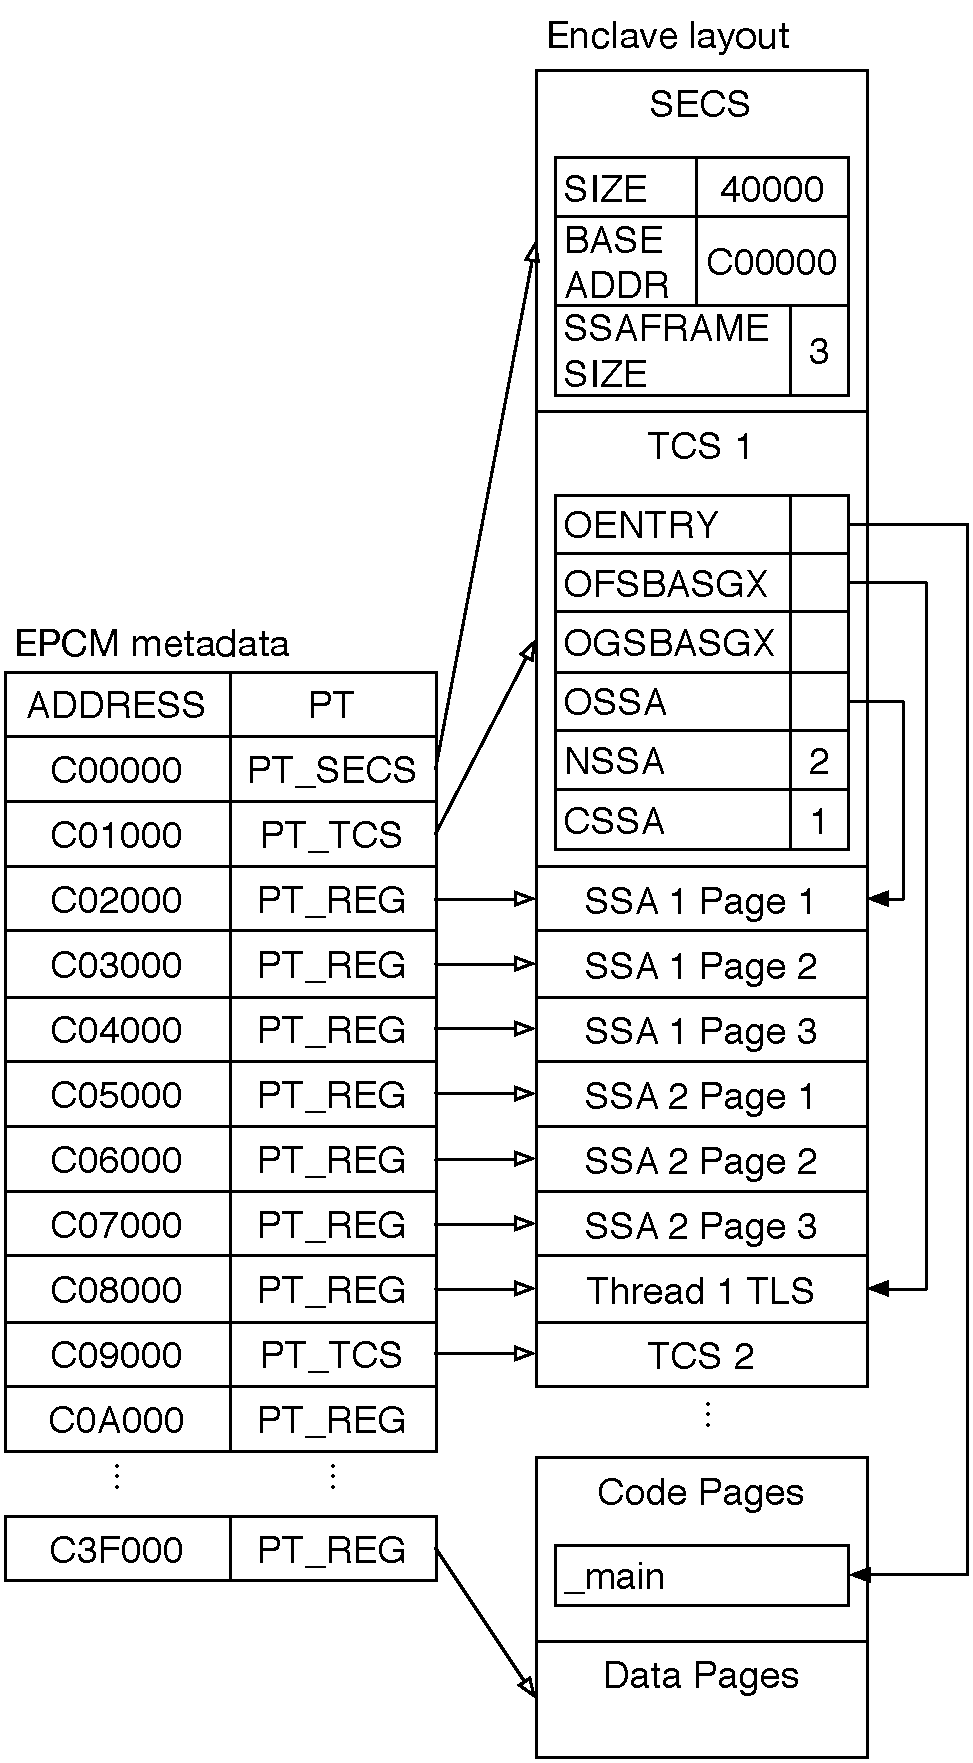
\includegraphics[width=70mm]{figures/enclave_layout.pdf}
  \caption{
    An enclave's memory layout. Each enclave has a SECS, and one TCS per
    supported hardware thread. Each TCS points to a sequence of SSAs, and
    specifies initial values for RIP, FS and GS.
  }
  \label{fig:enclave_layout}
\end{figure}

\subsubsection{The SGX Enclave Control Structure (SECS)}
\label{sec:secs}

% Main data structures: SGX/SGX2 S 1.4
% SECS: SGX S 2.6.1, S 2.6.1.1, SGX2 S 2.7, S 2.7.1, SGX/SGX2 S 3.1
% ECREATE: SGX/SGX2 S 3.1, S 5.3
% Implicit access: SGX/SGX2 S 2.5.3

The first step in creating an enclave is using the \texttt{ECREATE} instruction
to designate a previously unused EPC page as the enclave's \textit{SGX Enclave
Control Structure} (SECS). All instructions that operate on an enclave access
its control structure directly or indirectly.

% Internal CREGs: SGX2 S 5.1.4
% ECREATE: SGX2 S 5.3
% EWB: SGX2 S 5.3

The most important field in the SECS is the 64-bit \textit{enclave ID} (EID),
which is assigned by \texttt{ECREATE}. The EID identifies an enclave's pages in
the EPCM, so it must be unique across all the computer's active enclaves.
According to the ECREATE pseudo-code in the SDM, enclave IDs are allocated
using an atomic counter. An enclave's EID is generally hidden, as most SGX
instructions use the address of the enclave's SECS page as the enclave's
handler. However, the system software can learn an enclave's EID by evicting
one of its EPC pages (\S~\ref{sec:sgx_ewb}).

The software-visible SECS layout specifies the range of virtual addresses that
can be mapped to the enclave's EPC pages. Intel documentation calls the range
\textit{enclave linear address range} (ELRANGE). The range is specified using a
base (the BASEADDR field) and a size (the SIZE) field. ELRANGE must meet the
same constraints as a variable memory type range
(\S~\ref{sec:cacheability_config}), namely the size must be a power of 2, and
the base must be aligned to the size.

Currently, the main implication of ELRANGE is that all the SGX data structures
are initialized with enclave virtual addresses specified relatively to
BASEADDR. Furthermore, BASEADDR is not a part of the enclave's measurement
hash (details in \S~\ref{sec:measurement}). It follows that system software can
relocate an enclave in its host application's virtual address space, without
impacting the enclave's measurement hash.

Having ELRANGE follow the memory type range constraints provides a cheap way to
verify if a virtual address belongs to the address, in hardware. This provides
SGX engineers the option to implement per-enclave page tables in future SGX
revisions.

% SECS.ATTRIBUTES.XFRM: SGX/SGX2 S 6.7.2.1

The software-visible SECS has an ATTRIBUTE field that specifies the Intel
achitecture features used by the enclave code. For example, the MODE64BIT flag
is set if the enclave uses 64-bit code, and the XFRM sub-field contains the
XCR0 register value expected by the enclave's code. XCR0 controls Intel
architecture extensions such as SSE and AVX (see \S~\ref{sec:registers}).

When a logical processor executes code inside an enclave, it sets XCR0 to the
value specified by the enclave's SECS, so malicious system software cannot
enable features that the enclave code is not prepared to handle. This lets
Intel introduce extensions that change the architectural behavior of existing
instructions, such as Memory Protection Extensions (MPX), without having to
worry about introducing security vulnerabilities in SGX enclaves written before
MPX.

The other fields in the software-visible SECS layout are used by the
software attestation process, which is explained in \S~\ref{sec:attestation}.


\subsubsection{The Thread Control Structure (TCS)}
\label{sec:tcs}

% TCS: SGX S 2.6.2, S 2.6.2.{1,2,3,4}, SGX2 S 2.8, S 2.8.{1,2,3,4}

A logical processor uses a \textit{Thread Control Structure} (TCS) while
executing code inside an enclave, so enclave authors must provision at least as
many TCS instances as the number of concurrent software threads that they want
to use.

The fields in the software-visible TCS layout direct the context switches
performed by a logical processor when it transitions between non-enclave and
enclave code.

% SSA: SGX S 2.6.3, SGX2 S 2.9

In some cases (e.g., when receiving an interrupt), the processor needs to
preempt the execution of enclave code and start running kernel code. This is
accomplished by saving the enclave's context (register values) to an area
inside the enclave, called a \textit{State Save Area} (SSA).

Each TCS references a contiguous sequence of SSAs -- the OSSA field points to
the first SSA, and the NSSA field indicates the sequence's length. When a
logical processor needs to preempt enclave code, it uses the next available
SSA, indicated by the CSSA field in the TCS. The CPU refuses to execute enclave
code using a TCS where no SSA is available (CSSA $\ge$ NSSA).

An SSA essentially consists of the values of the general-purpose registers
(GPRs), and the result of running XSAVE (\S~\ref{sec:registers}) using the
feature mask specified in the ATTRIBUTES.XFRM field in the enclave's SECS.

% SECS.SSAFRAMESIZE: SGX/SGX2 S 6.7.2.2

Each SSA starts at the beginning of an EPC page, and takes up a fixed number of
EPC pages, specified in the SSAFRAMESIZE field in the enclave's SECS. The SSA
alignment and size restrictions most likely exist to simplify the SGX
implementation.

The TCS is stored in a page whose EPCM entry has the type PT\_TCS, and
therefore cannot be directly accessed by enclave software. However, SSAs are
stored in regular pages, so they are accessible to enclave software, and their
layout is defined in the SGX documentation.

\subsubsection{The Version Array (VA)}
\label{sec:va}

SGX includes support for system software to evict any EPC page to non-EPC RAM,
making it possible to have enclaves whose memory requirements exceed the
computer's EPC size. This is similar to ``swapping'', where the kernel evicts
pages of RAM to a hard disk while they are not accessed.

% VA: SGX S 2.6.12
% EPC and Management of EPC Pages: SGX S 3.5, 3.5.{2,3,4,5,6}

The EWB instruction evicts an EPC page to non-EPC memory. In the process, it
creates an 8-byte nonce (called \textit{page version} in the Intel
documentation), which must be stored in an unused slot of a \textit{Version
Array} (VA). Evicted pages are brought back into the EPC by the ELDU and ELDB
instructions, which use the nonce produced by EWB, and clear the VA slot that
held the nonce.

System software uses the EPA instructions to mark an unused EPC page as a VA.
Pages that store VAs have the PT\_VA EPCM type, so the nonces generated by EWB
cannot be read, even by enclave software.  A VA page has 512 8-byte slots.
Unused slots are marked by the value 0 (zero), and EPA zeroes out the EPC page
used to store the VA.

Non-EPC memory can be accessed by system software, which is untrusted in the
SGX threat model, so EWB (illustrated in Figure~\ref{fig:sgx_ewb}) encrypts and
MACs the contents of the EPC page before storing it in untrusted memory. The
nonces stored in VA pages prevent replay attacks where malicious system
software would attempt to bring back an old version of an evicted EPC page.


\subsection {The Implementation of EPC Protection}

The memory controller is
integrated on the CPU die (see Figure~\ref{fig:cpu_die}), so it can be trusted
to prevent devices attached to the system bus from performing DMA transfers
to/from the PRM.

System software manages physical memory by directly modifying the contents of
page tables and EPTs (\S~\ref{sec:paging}), and is responsible for performing
TLB shootdowns (\S~\ref{sec:tlbs}) to ensure that the state not covered by
cache coherence \S~\ref{sec:cache_coherence} is synchronized across logical
processors. If the system software does not perform TLB shootdowns correctly,
application software can experience inconsistent views of memory.

In the context of SGX, an incorrect TLB shootdown can can result in having an
EPC page simultaneously accessible by two different enclaves, which would
compromise the SGX security guarantees. Therefore, the SGX instructions used
for EPC management ensure that the system software performs TLB shootdowns for
the entries that represent EPC pages.

